

\textbf{Problem 2:}

We may extend the above problem with more general patterns of deadline
misses. Such patterns may be represented as infinite strings over the alphabet {0, 1},
such as $111011101110 \dots$, where a $1$ denotes that the corresponding
message instance meets its deadline constraint and $0$ denotes that the corresponding 
message instance misses its deadline constraint.

Based on a control-theoretic analysis, we can compute the set of all possible
such infinite strings which denote deadline miss patterns corresponding to which
given control performance constraints are satisfied. Let such a set of strings be
given by the language $L_{controller}$.

Similarly, given a platform, as in the case of Problem 1, let infinite strings
over the alphabet ${0, 1}$ denote transmission times of message instances over a
shared communication bus. Here, again, $1$ denotes that the corresponding message
instance meets its deadline constraint and $0$ denotes that the corresponding
message instance misses its deadline constraint. Such strings may be computed
using standard schedulability analysis techniques or model checking techniques
that analyze the platform (or scheduling policy) at hand. Let the set of such
strings be denoted by the language $L_{platform}$ .
Clearly, if $L_{platform} \subseteq L_{controller}$ then the control performance requirements
are satisfied when the control application is implemented on the platform in a
distributed fashion.
Again, we may ask different questions in this setup.


Question (Verification): Given control performance constraints for each 
controller, and a platform, are all the constraints satisfied?

Question (Synthesis): Given control performance constraints for each controller,
and a mapping of the control tasks on a distributed architecture, synthesize
bus or/and processor schedules such that the performance constraints
are satisfied.

\begin{figure}
\begin{center}
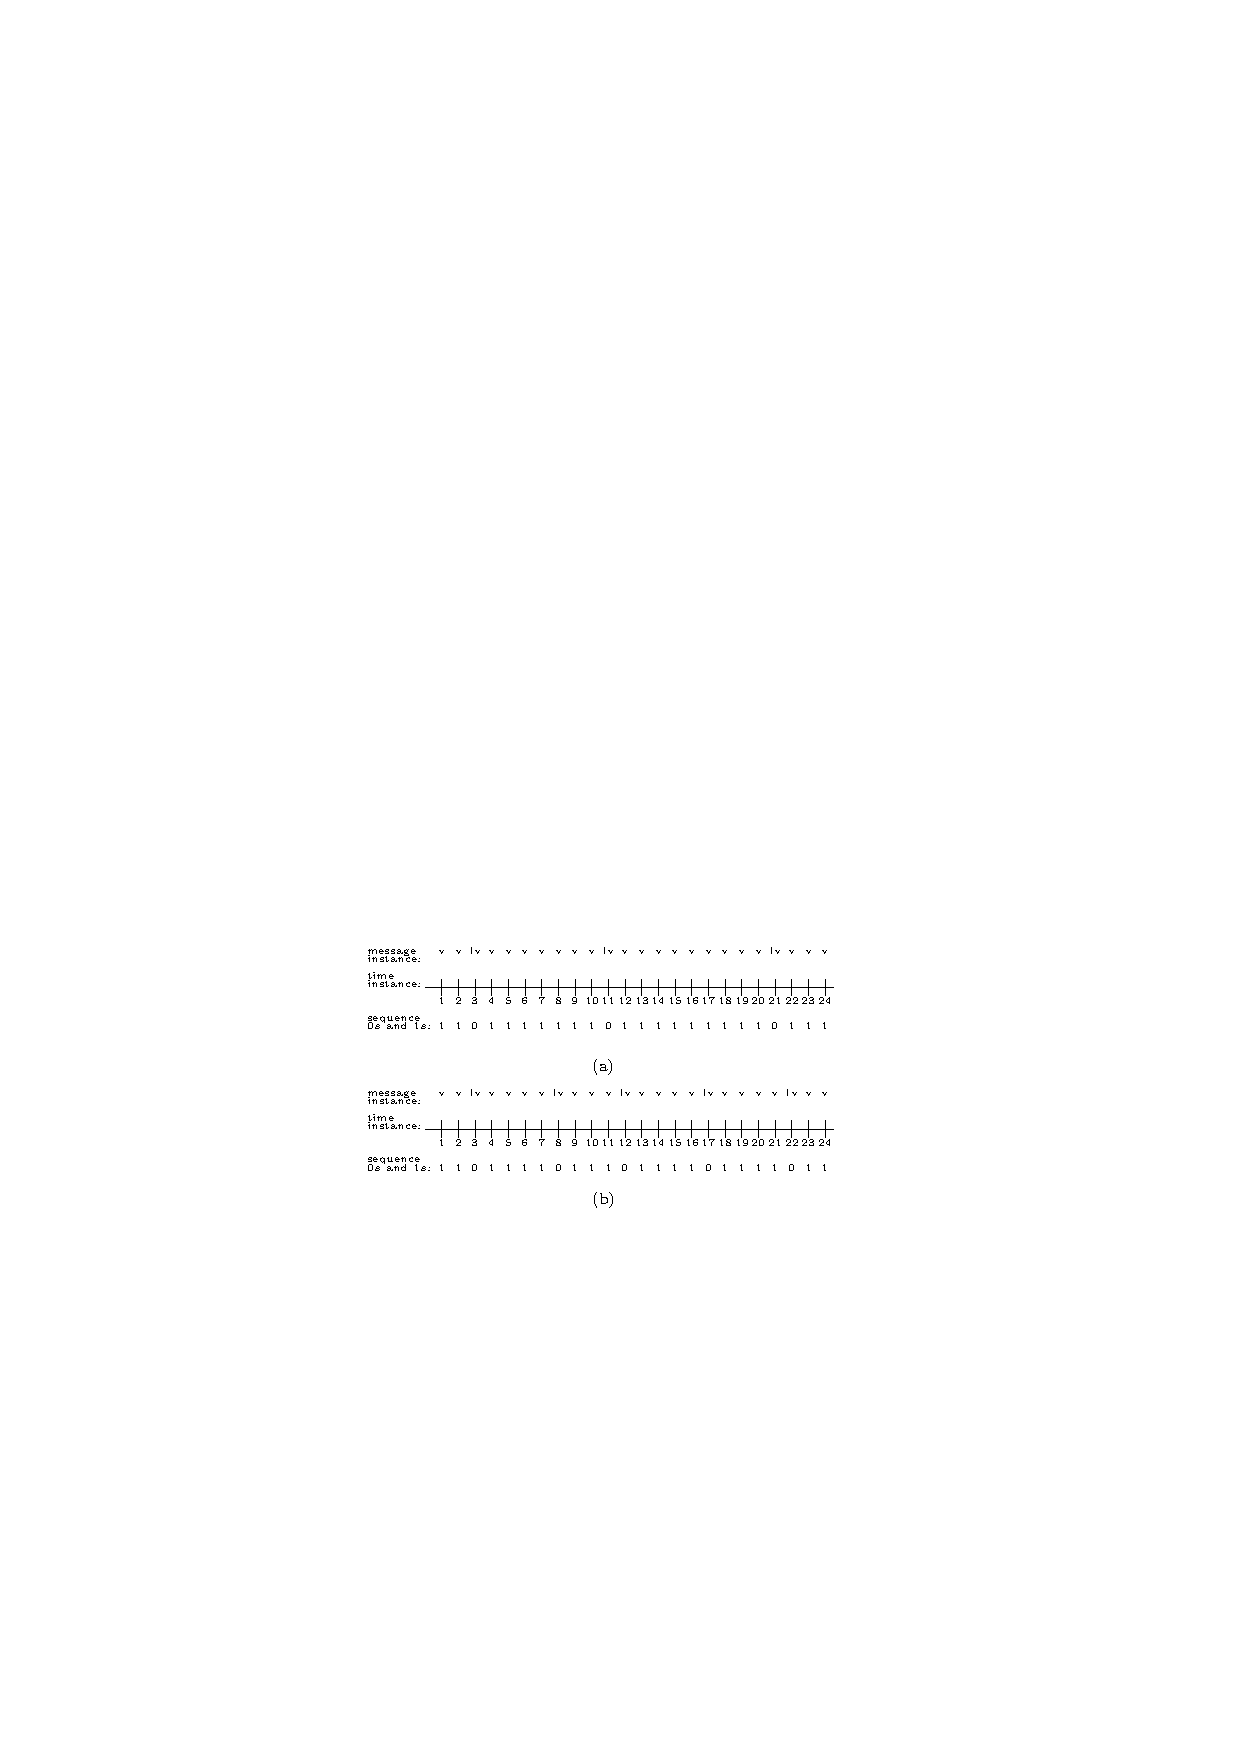
\includegraphics[width = 120mm]{vali_invalid_0_1.pdf}
\end{center}
\caption{Timing diagram}
\label{tim_dig_01}
\end{figure}

\textbf{Motivating Example:}
Let us consider the motivating example for Problem1. From the diagram Fig.\ref{tim_dig}, we  are representing
such valid-invalid sequence into streams of $0$ and $1$ where $1s$ represent valid massage
and $0s$ represent invalid messages. We considered that an invalid
message should be followed by at lest $k = 6$ valid messages. Now if we consider a $10$
length timing sample then possible satisfied combinations will be denoted by $L_{controller}
= \{ 0111111011, 1011111101,$ 

$1101111110, 0111111101, 0111111110, 1011111110, 0111111111, 1011111111, 1101111111,$ 

$1110111111, 1111011111, 1111101111, 11111101111, 11111110111, 11111111011, 1111111110\}$. Now if any $10$ 
length sequence satisfying the above condition will be any of the above mentioned sequence.
Any sequence other that these sequences will be vulnerable for the system.

In the Fig.\ref{tim_dig_01} the valid-invalid sequence is represented by streams of $0s$ and $1s$.
Now  we can say, that the sequence represented in Fig.\ref{tim_dig_01}(a) matches one
of the sequence but the sequence represented by Fig.\ref{tim_dig_01}(b) cannot match any of the 
satisfied sets of sequence. From Fig.\ref{tim_dig_01}(a), if we consider a $10$ length sequence
arbitrarily, say 7th slot to 16th slot. Here, $L_{platform} = 1111011111$ which is one of the
sequence present in $L_{controller}$, i.e, $L_{platform} \subseteq L_{controller}$. We can take
any of the $10$ length sequence and check the $L_{controller}$ set, then if the sequence is obeying
our satisfying constraint, then all of them will belong to that $L_{controller}$. But if it is not satisfying
like Fig.\ref{tim_dig_01}(b), we will get such sequence which does not belong to $L_{controller}$.


Solution Approach:
Instead of considering the full infinite sequence we can consider a window of size $w > (k + k/2)$. 
Because generating all possible sequence for infinite sequence will be itself a huge task.

For a given platform, if we have the satisfying constraint then we can get all of the valid
combinations of length $W$ satisfying the given constraint. If this window now passes through 
the infinite sequence and check whether it belongs to the valid set i.e, $L_{controller}$ , if 
we get valid sequence repeatedly then the system is safe. But if we get no match frequently, then 
from the safety property we can call the sequence as bad prefix.


